\section{User Interface}\label{sec:ui}
When the sensor data has arrived at the remote PC, the data has to be displayed. The data should be at least be output to a console. If possible due to time constraints, the data will be more visualised. In \ref{sec: Interfaces} the different implementations for the interfaces are discussed. In \ref{sec:Languages} the different options for the possible languages which can be used are discussed. In \ref{sec:rendering} the options for 3D-rendering are looked into.
\subsection{Interfaces}\label{sec: Interfaces}
\subsubsection{CUI}
The CUI (Console User Interface) is the most basic way the data will be output. All the sensor data will be output to the control with corresponding label. The CUI will automatically be updated when new data arrives. An example can be found in \ref{fig:CUI}.
\begin{figure}[H]
	\centering
	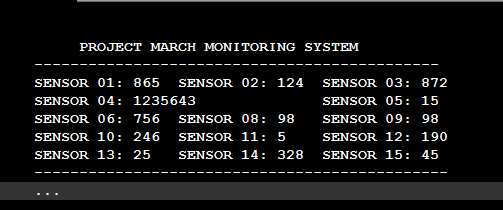
\includegraphics[width=.75\textwidth]{MockupCUI}
	\caption{A mock-up with a possible look of the CUI} 
	\label{fig:CUI}
\end{figure} 
\subsubsection{GUI}
The GUI (Graphic User Interface) consists of two parts. One part shows a dashboard with the most important sensor data visualised. The other part is a concise list with all sensor data. An example can be found in \ref{fig:GUI}  
\begin{figure}[H]
	\centering
	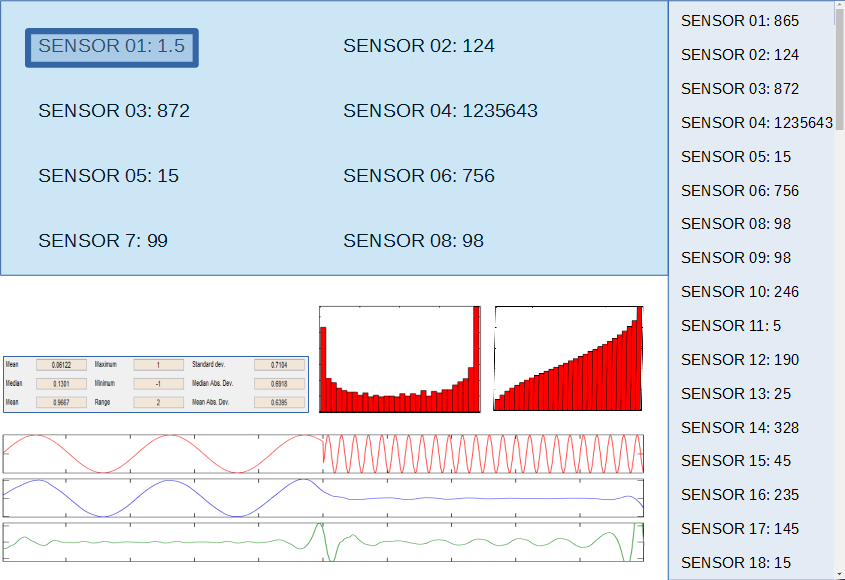
\includegraphics[width=.75\textwidth]{MockupGUI}
	\caption{A mock-up with a possible look of the GUI} 
	\label{fig:GUI}
\end{figure} 
\subsection{Languages}\label{sec:Languages}
For this project, it is important to use a language which has rich support for data visualisation and 3D-rendering. In addition, the chosen language must be able to (easily) interface Matlab since the sensor data will enter via a SimuLink model. In addition to the MATLAB language, C/C++, Java \& Python are valid options since Matlab has a build-in interface for these languages and these languages have libraries which support 3D-rendering and data visualisation. 
In the event that it proves to be impossible or undesirable to connect wireless directly using Matlab, there are three alternatives to consider corresponding with the network models in \ref{sec:impmod}. In the case of using the bridging models( \ref{sec:tbm} and \ref{sec:lbm}), Matlab will be used to create the GUI.
\\In the case of the Stand Alone model (\ref{sec:sm}), the option would be to use a stand-alone application which is based on another framework than Matlab. This would widen the range of possibilities for the use of the interface.
\\In the case of the Web Model (\ref{sec:wm}) the option is to create the GUI in HTML as a web-page and put a web-socket in the page to get the data. This implementation is very user friendly, as the only required software for the client is a web-browser. In addition, this makes it very easy for multiple people to use the monitoring system since the exoskeleton will broadcast over the wi-fi instead of sending the data directly to another client. By using this method, the options for the framework are limited to JavaScript and its libraries. In addition, running code in a browser tends to be less powerful than running the code in a stand-alone application. This might result in a lower update frequency and fewer options for data visualising.

\subsection{3D-Rendering}\label{sec:rendering}
Because of the fact that the 3D-rendering has shifted to a lower priority, less effort has been expended in researching suitable frameworks for rendering. Still, a small list have been compiled of some rendering frameworks which are simple to use for each of the narrowed down languages. In addition, Matlab contains build-in modules for 3D-rendering.
\begin{itemize}
	\item C/C++: Ogre3D \cite{web:ogre3d}
	\item Java/Scala: Env3D \cite{web:env3d}
	\item Python: Panda3D \cite{web:panda3d}
\end{itemize}
	